% ReRoom -- method overview (paper-figure style, submission-safe vector graphic).
\documentclass[border=6pt]{standalone}
\usepackage{tikz}\usepackage{amsmath,amssymb}\usepackage{pifont}
\usetikzlibrary{arrows.meta,positioning,fit,backgrounds,calc}
\definecolor{ink}{HTML}{1A1A1A}
\definecolor{mut}{HTML}{6B7280}
\definecolor{net}{HTML}{3B5BD9}
\definecolor{prj}{HTML}{E8770F}
\tikzset{
  lbl/.style   ={font=\scriptsize,text=ink},
  slbl/.style  ={font=\tiny,text=mut},
  stp/.style   ={draw=ink,line width=.5pt,rounded corners=1.5pt,fill=white,align=center,font=\scriptsize,inner sep=2.5pt,text=ink},
  netbox/.style={draw=net,line width=1pt,rounded corners=4pt,fill=net!4},
  prjbox/.style={draw=prj,line width=1pt,dashed,rounded corners=3pt,fill=prj!7,align=center,font=\scriptsize,text=ink,inner sep=3pt},
  main/.style  ={-{Stealth[length=5pt]},line width=1pt,ink},
  aux/.style   ={-{Stealth[length=3.5pt]},line width=.6pt,net},
  wall/.style  ={line width=1pt,ink},
}
\newcommand{\furn}[5]{\fill[#5,rounded corners=.4pt] (#1,#2) rectangle ++(#3,#4);}
\begin{document}
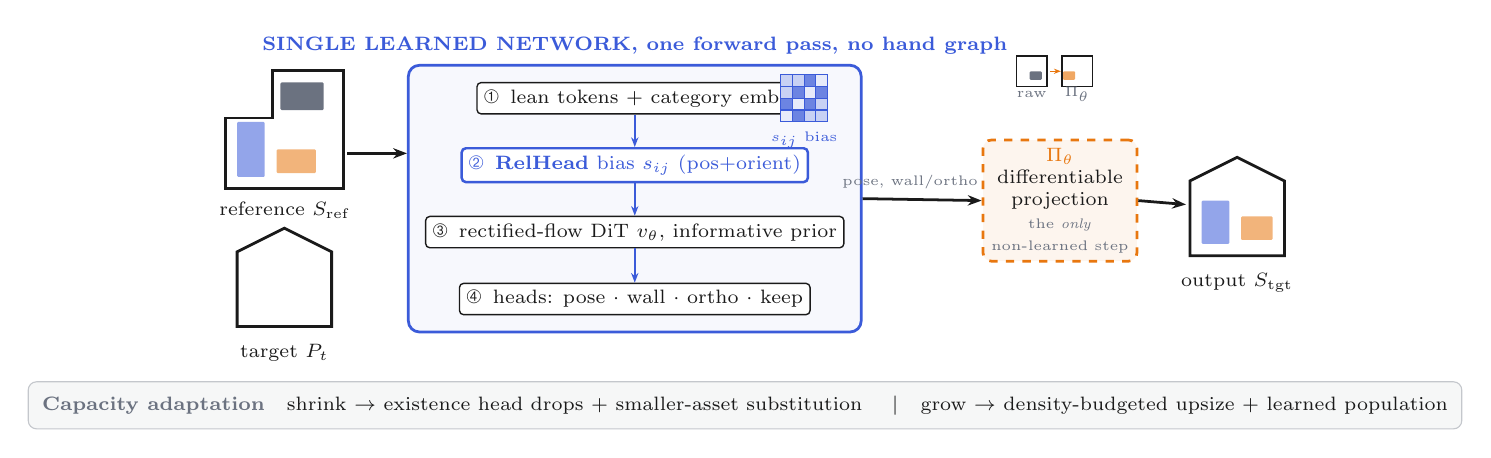
\begin{tikzpicture}
% 1. INPUT
\draw[wall] (0,0.2)--(1.5,0.2)--(1.5,1.7)--(0.6,1.7)--(0.6,1.1)--(0,1.1)--cycle;
\furn{0.15}{0.35}{0.35}{0.7}{net!55}\furn{0.65}{0.4}{0.5}{0.3}{prj!55}\furn{0.7}{1.2}{0.55}{0.35}{mut}
\node[lbl,below] at (0.75,0.15) {reference $S_\text{ref}$};
\draw[wall] (0.15,-1.55)--(1.35,-1.55)--(1.35,-0.6)--(0.75,-0.3)--(0.15,-0.6)--cycle;
\node[lbl,below] at (0.75,-1.65) {target $P_t$};
% 2. LEARNED NETWORK
\def\nx{5.2}
\node[stp,minimum width=30mm] (s1) at (\nx,1.35) {\ding{192}\, lean tokens $+$ category emb.};
\node[stp,text=net,draw=net,line width=.9pt,minimum width=30mm] (s2) at (\nx,0.5) {\ding{193}\, \textbf{RelHead} bias $s_{ij}$ (pos$+$orient)};
\node[stp,minimum width=30mm] (s3) at (\nx,-0.35) {\ding{194}\, rectified-flow DiT $v_\theta$, informative prior};
\node[stp,minimum width=30mm] (s4) at (\nx,-1.2) {\ding{195}\, heads: pose $\cdot$ wall $\cdot$ ortho $\cdot$ keep};
\draw[aux] (s1)--(s2); \draw[aux] (s2)--(s3); \draw[aux] (s3)--(s4);
\node (hm) at (7.35,1.35) {};
\begin{scope}[shift={(7.05,1.05)},scale=0.15]
  \foreach \i in {0,1,2,3}\foreach \j in {0,1,2,3}{
    \pgfmathsetmacro\v{abs(\i-\j)==1 ? 75 : (\i==\j?12:28)}
    \fill[net!\v] (\i,\j) rectangle ++(1,1);}
  \draw[net,line width=.4pt] (0,0) grid (4,4);
\end{scope}
\node[slbl,text=net] at (7.35,0.82) {$s_{ij}$ bias};
\begin{scope}[on background layer]
  \node[netbox,fit=(s1)(s2)(s3)(s4)(hm),inner sep=6pt,label={[net,font=\scriptsize\bfseries]above:SINGLE LEARNED NETWORK, one forward pass, no hand graph}] (net) {};
\end{scope}
% 3. Pi_theta
\node[prjbox,minimum width=18mm] (pi) at (10.6,0.05) {\textbf{\textcolor{prj}{$\Pi_\theta$}}\\ differentiable\\ projection\\ {\tiny\color{mut} the \emph{only}}\\ {\tiny\color{mut} non-learned step}};
\begin{scope}[shift={(10.05,1.5)},scale=0.55]
  \draw[wall,line width=.5pt] (0,0) rectangle (0.7,0.7);
  \furn{0.30}{0.15}{0.28}{0.2}{mut}\node[slbl] at (0.35,-0.18){raw};
  \draw[wall,line width=.5pt] (1.05,0) rectangle (1.75,0.7);
  \furn{1.07}{0.15}{0.28}{0.2}{prj!65}\node[slbl] at (1.40,-0.18){$\Pi_\theta$};
  \draw[prj,-{Stealth[length=2.5pt]},line width=.5pt] (0.78,0.35)--(1.02,0.35);
\end{scope}
% 4. OUTPUT
\draw[wall] (12.25,-0.65)--(13.45,-0.65)--(13.45,0.3)--(12.85,0.6)--(12.25,0.3)--cycle;
\furn{12.4}{-0.5}{0.35}{0.55}{net!55}\furn{12.9}{-0.45}{0.4}{0.3}{prj!55}
\node[lbl,below] at (12.85,-0.75) {output $S_\text{tgt}$};
% arrows
\draw[main] (1.55,0.65) -- (net.west|-{(0,0.65)});
\draw[main] (net.east) -- (pi.west) node[pos=0.4,above,slbl]{pose, wall/ortho};
\draw[main] (pi.east) -- (12.2,0.0);
% capacity
\node[draw=mut!40,fill=mut!6,rounded corners=3pt,align=center,font=\scriptsize,inner sep=5pt,text=ink,minimum width=134mm] (cap) at (6.6,-2.55) {\textbf{\textcolor{mut}{Capacity adaptation}}\quad shrink $\to$ existence head drops $+$ smaller-asset substitution \quad$\vert$\quad grow $\to$ density-budgeted upsize $+$ learned population};
\end{tikzpicture}
\end{document}
